---
title: TikZ 自動変換のテスト
date: 2014/03/23 21:59:06 JST
author: 石井大海
description: description
tag: TeX
---

\documentclass[dvipdfmx,uplatex,a4j]{jsarticle} % say
\usepackage{tikz}
\usetikzlibrary{matrix,arrows}
\begin{document}

直積のアレが下のそれです:
\begin{center}
 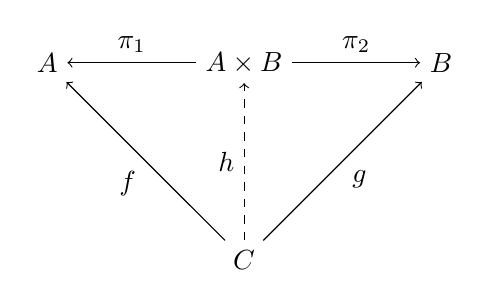
\begin{tikzpicture}[node distance=2.5cm, auto]
 \node (A) {$A$};
 \node (AB) [right of=A] {$A \times B$};
 \node (B)  [right of=AB] {$B$};
 \node (C)  [below of=AB] {$C$};
 \draw[->] (AB) to node [swap] {$\pi_1$} (A);
 \draw[->] (AB) to node {$\pi_2$} (B);
 \draw[->] (C)  to node {$f$} (A);
 \draw[->] (C)  to node [swap] {$g$} (B);
 \draw[->, dashed] (C) to node {$h$} (AB);
 \end{tikzpicture}
\end{center}

ほえー,なんか直積っぽい.
\end{document}
